\documentclass{article}
\usepackage[T1]{fontenc}
\usepackage[utf8]{inputenc}
\usepackage{microtype}
\usepackage{graphicx}
\usepackage{booktabs,tabularx,multirow,array}
\usepackage{amsmath,amssymb,amsthm,mathtools}
\usepackage{xcolor}
\usepackage{xurl}
\usepackage{hyperref}
\usepackage{mlsys2025}
\usepackage{enumitem}
\newcommand{\famp}{\textsc{Famp}}
\newcommand{\E}{\mathbb{E}}
\newcommand{\R}{\mathbb{R}}
\newcommand{\ind}{\mathbf{1}}
\newcommand{\bytes}{\operatorname{bytes}}
\newcommand{\risk}{\mathcal{R}}
\newcommand{\blank}{\phantom{00.00}}
\newcommand{\RQ}[1]{\textbf{RQ#1}}
\newcommand{\code}[1]{\texttt{\small #1}}
\newtheorem{proposition}{Proposition}
\newtheorem{definition}{Definition}
\newcolumntype{Y}{>{\raggedright\arraybackslash}X}
\hypersetup{pdfauthor={Anonymous authors},pdfsubject={Research draft; confirmatory tables intentionally empty}}
\mlsystitlerunning{FAMP: Executable Memory for Byte-Budgeted Continual Learning}

\begin{document}
\twocolumn[
\mlsystitle{FAMP: Diagnosis-Guided Executable Memory\\for Byte-Budgeted Continual Learning}
\begin{mlsysauthorlist}
\mlsysauthor{Anonymous Authors}{anon}
\end{mlsysauthorlist}
\mlsysaffiliation{anon}{Anonymous Institution}
\mlsyscorrespondingauthor{Anonymous Author}{anonymous@example.com}
\mlsyskeywords{continual learning, functional memory, modular reuse, replay, resource budgets, selective admission}
\vskip 0.3in
]
\printAffiliationsAndNotice{}
\begin{abstract}
A continual learner can retain examples, model parameters, or constraints on future updates, but these representations have different storage and execution costs. Replacing examples with purportedly reusable knowledge is beneficial only when the retained computation, its task interfaces, and its verification state are cheaper at competitive accuracy. We present \famp{}, a task-incremental learner that makes this replacement explicit. A mutable fallback model learns each task with residual replay. A bounded search proposes reusing an immutable feature unit, composing existing units, or allocating a compact learned unit. Independent acceptance data test harmful disagreements with the fallback teacher and consistency under declared input perturbations. A byte-accounted transaction publishes an executable route only after these checks and then removes the covered task's ordinary episodes. Rejection preserves the fallback path. We derive a conditional excess-risk bound for admission and a persistent-state invariant, while separating architectural immutability from semantic abstraction. The implementation exposes physical sharing, per-object storage, discovery overhead, and inference costs. A research-question-driven protocol distinguishes the value of memory substitution from independent task isolation, ordinary distillation, compressed replay, and permissive reuse. This draft leaves confirmatory result cells empty; no resource or accuracy advantage is assumed.
\end{abstract}

\section{Introduction}
Continual learning must reconcile acquiring new capabilities with retaining earlier ones. For a resource-constrained implementation, the problem is not only which parameters to update, but also \emph{what to retain between tasks}. Episodic replay stores observations; distillation may additionally store predictions; modular methods retain reusable parameters; gradient methods retain directions that constrain adaptation. Each representation consumes bytes and requires computation to maintain or execute. Accounting only for an example count can therefore reverse the apparent ranking of methods when model copies, logits, and auxiliary state are included \cite{buzzega2020,seo2024}.

\begin{figure*}[t]
\centering
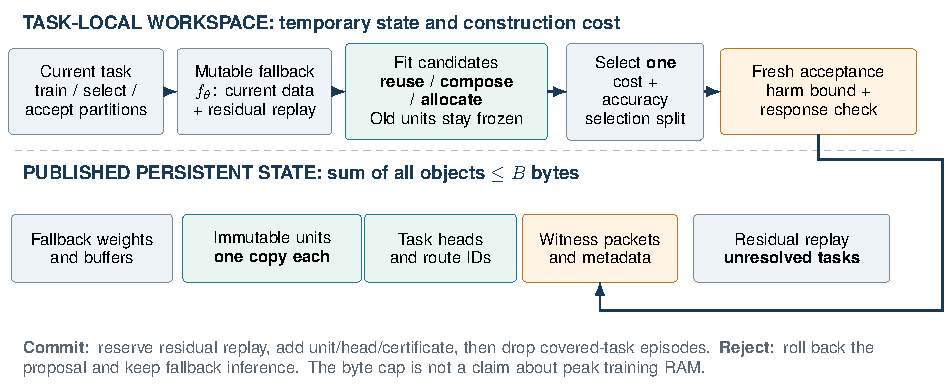
\includegraphics[width=\textwidth]{figures/01_system.pdf}
\caption{\textbf{A storage representation is selected, not merely an update penalty.} The task-local workspace contains the mutable learner and candidate-fitting computations. The published state is separately byte-accounted. Only one proposal reaches independent acceptance. A successful transaction stores the complete executable route and bounded witnesses, then removes ordinary episodes for that task. Otherwise the task remains on the mutable fallback. Temporary workspace and rejected-candidate time are costs, not part of a hidden ``free'' memory allowance.}
\label{fig:system}
\end{figure*}

The motivating hypothesis is that some task experience can be replaced by a compact executable computation shared with later tasks. This is more specific than retaining a stable activation pattern. A stored gradient direction describes update sensitivity but is not an executable skill. Conversely, a small feature vector is not a self-contained computation unless the encoder, decoder, and interface needed to use it remain available. The relevant comparison is thus between complete retained representations, not between an image buffer and an isolated vector.

Modular reuse itself is established. Progressive networks protect earlier columns; PackNet packs tasks through pruning; compositional lifelong learning separates the combination of existing components from their adaptation; and MNTDP searches for reusable modules using task-driven priors \cite{rusu2016,mallya2018,mendez2021,veniat2021}. These results motivate, rather than establish, the benefit of an explicit \emph{memory-substitution decision}. A new task-specific head may make a frozen unit useful, yet selecting that unit because it is cheap can lock in an inadequate predictor. Keeping both the unit and an unchanged episode buffer can eliminate any storage benefit. Finally, a counterfactual or feature-similarity score does not by itself justify treating a candidate as a reusable mathematical abstraction \cite{geiger2022,geiger2024}.

\famp{} addresses the narrower systems question: \emph{when should a task's ordinary episodes be replaced by a byte-accounted executable route through learned units?} It combines a mutable replay learner with an immutable unit store. The controller diagnoses whether a task can use existing units, needs a new unit, or should remain on the fallback path. Here ``diagnosis'' denotes an evidence-backed \emph{allocation decision}, not identification of a unique physical cause of forgetting. Existing units are not altered when a new head is fitted. The controller separates candidate selection from independent acceptance and records every rejected proposal, including its construction cost.

The proposed contribution is the interaction of three design choices: a transactional replacement of episodic state by shared executable objects; an independent teacher-relative admission check supplemented by perturbation-response consistency; and complete accounting of the weights, task heads, certificates, metadata, and fallback needed to operate the learner. None of modularity, distillation, confidence bounds, or total-byte accounting is claimed as individually new. The decisive empirical question is whether this combination improves the resource--accuracy trade-off \emph{beyond} compressed replay and otherwise identical non-sharing units.

This paper fixes the algorithm and a falsifiable evaluation protocol. The code executes a development pilot, but its measurements are kept in a separate report rather than entered into the confirmatory tables. The distinction is important: observing an immutable path or a shared unit identifier validates implementation behavior; it does not establish lower memory at matched accuracy, lower training cost, or a general abstraction-learning result.



\section{Problem and Retention Contract}
\label{sec:problem}
\subsection{Task-incremental learning}
A stream contains tasks $t=1,\ldots,T$, each with distribution $P_t(x,y)$ and a supplied task identifier. Training is task-batch continual learning: the current task's training partition is available during its stage, whereas past training examples are accessible to the learner only through retained memory. Inference receives $(x,t)$. This is not task-agnostic class-incremental classification. All task-specific heads, identifier-dependent parameters, and route metadata count toward storage.

Each task provides disjoint training, selection, acceptance, and test partitions. Training fits model parameters; selection chooses a proposal; acceptance decides whether to publish it; the test partition is read only by the observer. A fresh acceptance set is required for each attempted task admission. Synthetic primitive values belong to the data generator and observer, not the optimizer. Declared perturbations produce alternate inputs without requesting new labels. For images these are augmentation responses, not ground-truth semantic interventions.

The persistent state after task $t$ is
\begin{equation}
\mathcal{S}_t=(\theta_t,\mathcal{U}_t,\mathcal{H}_t,\mathcal{I}_t,
                    \mathcal{V}_t,\mathcal{E}_t,\mathcal{J}_t),
\end{equation}
where $\theta_t$ parameterizes the mutable fallback, $\mathcal{U}_t$ is the immutable unit bank, $\mathcal{H}_t$ contains task heads, $\mathcal{I}_t$ maps tasks to unit identifiers, $\mathcal{V}_t$ contains bounded witnesses and admission statistics, $\mathcal{E}_t$ is residual episodic memory, and $\mathcal{J}_t$ is serialization metadata. The retention contract is $\bytes(\mathcal{S}_t)\le B$ at every published task boundary. A separate peak-workspace measurement captures gradients, optimizer state, candidate copies, and transient tensors. The two quantities are not interchangeable.

\subsection{What constitutes a functional unit?}
\begin{definition}[Executable functional unit]
A unit $U_k$ is a deterministic learned map from a declared, fixed input representation to a feature vector, together with all parameters and immutable buffers required to execute that map. A task route consists of unit identifiers and a learned head $h_t$; it is closed if its execution has no dependency on mutable fallback parameters.
\end{definition}
In the prototype, units consume raw preprocessed inputs and output eight features. A route can reference one or two units:
\begin{equation}
\hat f_t(x)=h_t\!\left(\mathop{\Vert}_{k\in I_t} U_k(x)\right),\qquad |I_t|\le2,
\label{eq:route}
\end{equation}
where $\Vert$ denotes concatenation. Uncovered tasks use $f_{\theta_t}(x,t)$. A shared unit is a single physical parameter object referenced by at least two task routes, not two independently fitted objects with similar outputs.

This definition deliberately stops short of a symbolic abstraction. An eight-dimensional encoder can carry entangled information and its head can implement a task-specific decision. We therefore distinguish \emph{executable sharing}, \emph{teacher-consistent substitution}, and \emph{semantic abstraction}. The first two are testable system properties here. A proof of the third would require stronger causal models and intervention coverage than a finite teacher-consistency check \cite{geiger2024}.

\subsection{Success is a constrained resource trade-off}
Let $A_{t,j}$ be task $j$'s accuracy after stage $t$. Final accuracy, acquisition, and max-based forgetting are reported separately:
\begin{align}
A_{\mathrm{final}}&=T^{-1}\textstyle\sum_j A_{T,j},\\
A_{\mathrm{acq}}&=T^{-1}\textstyle\sum_j A_{j,j},\\
F&=(T-1)^{-1}\textstyle\sum_{j<T}\left[\max_{k=j,\ldots,T} A_{k,j}-A_{T,j}\right].
\end{align}
For reordered streams, acquisition indices replace the task labels in these expressions. Including the final checkpoint in the maximum makes $F$ nonnegative; backward transfer is also reported so that improvements after acquisition are visible \cite{lopez2017}.

The primary systems comparison is the smallest \emph{measured} budget achieving a validation-selected target accuracy within a predeclared tolerance, followed by independent test evaluation. The selected method must also satisfy acquisition and forgetting tolerances. We do not infer a memory improvement from fewer episodes if units and interfaces consume the saved bytes. Likewise, construction overhead is not justified by an unchanged test score unless another measured resource improves.

\section{FAMP Design}
\label{sec:design}
\subsection{Mutable fallback and immutable published routes}
The fallback is a task-conditioned neural classifier trained with current examples and bounded residual replay. It is shared by all primary implementations, including replay-only baselines. The fallback continues to learn unresolved tasks after other tasks have been published as immutable routes. This separation preserves an escape path when a compact representation is insufficient: rejection is an ordinary operating mode, not a failed run discarded from evaluation.

A compact unit is learned from the current task rather than supplied as an arithmetic program. Its training combines task cross-entropy with soft-target distillation from the fallback frozen for the duration of candidate fitting:
\begin{equation}
\begin{aligned}
\mathcal{L}_{U,h}={}&\E_{(x,y)\in D_t^{\mathrm{tr}}}\ell(h(U(x)),y)\\
&+\lambda T_d^2\E_{x\in D_t^{\mathrm{tr}}}
 D_{\mathrm{KL}}(p_\theta^{T_d}(x)\Vert p_{U,h}^{T_d}(x)).
\end{aligned}
\label{eq:distill}
\end{equation}
$T_d$ is distillation temperature, distinct from the task horizon. Distillation is standard \cite{hinton2015}; its role is to construct a compact executable candidate, not to provide an uncounted persistent teacher. The current fallback itself serves as teacher, and no additional teacher copy survives publication.

\subsection{Bounded search and the operational diagnosis}
For a new task, the controller considers at most the three most recently admitted units, each with a newly fitted head, a concatenation of the two most recent eligible units, and one newly trained unit. Recency is a disclosed bounded heuristic; it does not inspect hidden task similarities or numerical primitives. Existing unit weights are frozen while the corresponding heads are trained. Candidate feature caches are temporary and their time and workspace belong to the construction phase.

On $D_t^{\mathrm{sel}}$, a candidate is eligible if its accuracy is within a selection slack of the current teacher. The proposal minimizes incremental parameter bytes among eligible candidates, breaking ties by selection accuracy. Witness and metadata bytes are determined and charged in the subsequent transaction. This is a bounded local selection policy, not a globally optimal dictionary learner: an immediately cheap candidate may prevent useful future consolidation, and the recency shortlist can miss an older reusable unit.

The resulting diagnosis is one of \emph{reuse}, \emph{compose}, \emph{allocate}, or \emph{fallback}. It records whether the obstacle was selection accuracy, teacher competence, excess-harm uncertainty, perturbation mismatch, or the byte cap. It does not infer a unique cause such as ``routing damage'' from representation alignment. That restriction avoids making the storage policy depend on an unverified causal attribution.

\begin{algorithm}[t]
\caption{One FAMP task-boundary transaction}
\label{alg:famp}
\begin{algorithmic}[1]
\REQUIRE Current task partitions; published state $\mathcal S$; cap $B$
\STATE Train fallback on $D_t^{\mathrm{tr}}$ and retained $\mathcal E$
\STATE Construct bounded reuse, composition, allocation proposals
\STATE Fit candidates using $D_t^{\mathrm{tr}}$ only
\STATE Select one eligible proposal $g$ using $D_t^{\mathrm{sel}}$
\IF{no proposal is eligible}
\STATE Retain bounded episodic state; return fallback
\ENDIF
\STATE Compute excess-harm bound and response check on $D_t^{\mathrm{acc}}$
\IF{teacher, risk, or response check fails}
\STATE Discard proposal; retain bounded replay; return fallback
\ENDIF
\STATE Stage unit references, head, witnesses, and metadata
\STATE Reserve residual replay for currently unresolved tasks
\IF{staged persistent state exceeds $B$}
\STATE Roll back staged objects; return fallback
\ENDIF
\STATE Publish closed immutable route; remove task-$t$ ordinary episodes
\STATE Rebalance residual replay; assert exact byte ledger
\STATE Verify older route witnesses; return published state
\end{algorithmic}
\end{algorithm}

\subsection{Independent admission and response consistency}
Only the selected proposal accesses $D_t^{\mathrm{acc}}$. Let $g_t$ denote the candidate and $f_t$ the frozen current teacher. Define the harmful-disagreement event
\begin{equation}
H(x,y)=\ind\{f_t(x)=y\ \land\ g_t(x)\ne y\}.
\label{eq:harm}
\end{equation}
For $n$ IID acceptance examples with $k$ such events, we compute the one-sided Clopper--Pearson upper bound
\begin{equation}
U(k,n,\alpha_t)=
\begin{cases}
\operatorname{Beta}^{-1}(1-\alpha_t;k+1,n-k),&k<n,\\
1,&k=n.
\end{cases}
\label{eq:cp}
\end{equation}
This standard confidence construction is attributed to \citet{clopper1934}. Admission requires $U\le\epsilon$ and a minimum observed teacher accuracy. The latter is a competence screen, not an independent theorem about absolute teacher risk.

Image acceptance sets are stratified by class. A pooled binomial bound would incorrectly treat those trials as identically distributed. Instead, with $C$ classes and declared class weights $\pi_c$, FAMP uses
\begin{equation}
U_{\mathrm{strat}}=\sum_{c=1}^C\pi_c U(k_c,n_c,\alpha_t/C).
\label{eq:strat}
\end{equation}
An unobserved class receives upper bound one. Equal class weights match the balanced task evaluation. This correction can make small datasets unsuitable for confident substitution; the controller must reject rather than recycle acceptance labels into training or silently relax its threshold.

The second check compares probability responses under declared label-free perturbations $\tau$:
\begin{align}
\Delta_f(x,\tau)&=p_f(\tau(x))-p_f(x),\\
D_{\mathrm{resp}}(g,f)&=
 \left[\E_{x,\tau}\|\Delta_g(x,\tau)-\Delta_f(x,\tau)\|_2^2/C\right]^{1/2}.
\label{eq:response}
\end{align}
The prototype evaluates four seeded perturbations and requires $D_{\mathrm{resp}}\le\eta$. Synthetic perturbations change one raw operand pair, including a nuisance pair; image perturbations mildly attenuate a row or alter intensity. No transformed labels are requested. Consequently this is a \emph{teacher-response consistency gate}, not proof that the unit computes comparison, multiplication, or another named operation. Structured pairs carry additional information and must not be equated with unrestricted unsupervised discovery \cite{locatello2020}.

\begin{figure*}[t]
\centering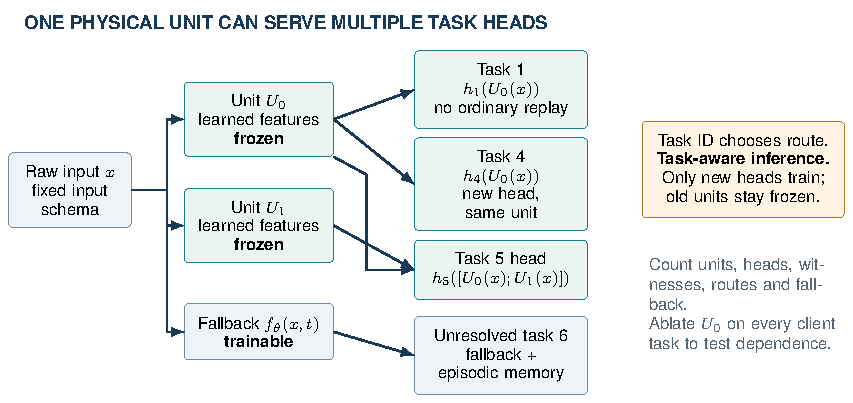
\includegraphics[width=\textwidth]{figures/02_executable_reuse.pdf}
\caption{\textbf{A closed executable graph makes sharing auditable.} Unit $U_0$ is stored once and consumed by several frozen task heads; another head composes two units. Unresolved tasks continue through a mutable fallback. The task ID selects the route. Because every unit starts from fixed raw preprocessing, there is no mutable shared encoder whose drift invalidates old routes. A unit ablation tests dependence across its actual clients, but does not establish a uniquely interpretable symbolic function.}
\label{fig:reuse}
\end{figure*}

\subsection{Publication, rollback, and residual replay}
The transaction stages the candidate's new unit, if any, its head, route identifiers, admission statistics, and a fixed-size witness packet. It computes the full prospective ledger and reserves a minimum episodic slice for tasks unresolved \emph{at that boundary}. This reservation is not a guarantee of a fixed per-task episode count for an unbounded future stream. If the cap is exceeded, staged objects are removed and their references restored; no earlier published unit is evicted or modified.

After a successful publication, ordinary task-$t$ training examples are omitted from episodic memory. The retained witness packet contains a few encoded inputs, labels, teacher targets, and perturbation seeds; these are counted as stored data, not described as zero-replay learning. Residual replay is balanced over task/class queues using priorities assigned while the relevant data are available. Previously discarded old examples never re-enter from an archived historical dataset.

The immutable design prevents interference through admitted routes but limits adaptation: a frozen error also remains frozen, and an improved fallback does not automatically upgrade old heads. Selective revision, unit eviction, and automatic task inference are outside this version. In particular, publishing more routes is not inherently better. The ungated ablation tests whether low storage can be obtained merely by permanently accepting poor predictors.

\section{Guarantees, Limits, and Cost Model}
\label{sec:analysis}
\begin{proposition}[Conditional admission risk]
Condition on the training/selection history and a proposal fixed before its acceptance data are observed. Under IID acceptance sampling, with probability at least $1-\alpha_t$, an admitted candidate satisfies
$\risk_{P_t}(g_t)-\risk_{P_t}(f_t)\le\epsilon$.
For class-stratified data the same statement follows from Eq.~\eqref{eq:strat}, assuming independent sampling within each class and the declared mixture weights.
\end{proposition}
\begin{proof}
Pointwise, $\ind\{g_t(x)\ne y\}-\ind\{f_t(x)\ne y\}\le H(x,y)$: a candidate can add an error only when the teacher was correct. Taking expectations gives $\risk(g_t)-\risk(f_t)\le\E H$. The binomial upper confidence bound covers $\E H$ with failure probability at most $\alpha_t$. Accepting only when it is at most $\epsilon$ proves the statement. In stratified sampling, apply the bound within each class and a union bound, then weight the class risks.\end{proof}
Using $\alpha_t=\alpha/T$ gives an at-most-$\alpha$ probability of any incorrectly bounded admission over the declared finite horizon. Candidate search does not invalidate the result because acceptance is independent and only one selected candidate is tested per task. Repeated attempts on the same acceptance data would invalidate this reasoning without additional correction. The guarantee is teacher-relative and distribution-specific; it is neither an absolute accuracy guarantee nor protection from distribution shift.

\begin{proposition}[Closed-route persistence]
If a published route's preprocessing, units, head, and buffers are immutable, then its output is unchanged by any subsequent optimization of the fallback or disjoint candidate objects, apart from numerical execution variation.
\end{proposition}
This follows by substituting unchanged functions into Eq.~\eqref{eq:route}. The property concerns retained computation, not learned semantic identity, and is related to earlier parameter-isolation methods \cite{rusu2016,mallya2018}. The implementation checks it on bounded witnesses and by hashing published units. Witness agreement is an implementation test; closure of the dependency graph supplies the structural argument.

\begin{proposition}[Published-state budget]
If $\bytes(\mathcal S_0)\le B$ and each admission publishes only a byte-checked staged state, while residual replay is trimmed to the remaining capacity, then $\bytes(\mathcal S_t)\le B$ at every published boundary.
\end{proposition}
The proof is induction over committed and rejected transactions. A rejection leaves the unit store unchanged; a commit is explicitly checked before publication; replay uses only residual capacity. The result does not bound peak training allocation or external artifact files. Those must be measured separately.

For base bytes $W_0$, unique unit bytes $W_k$, task-interface bytes $A_t$, witness/metadata bytes $V_t$, and episodic record size $b_e$, the ledger is
\begin{equation}
S=W_0+\sum_{k\in\mathcal U}W_k+\sum_{t\in\mathcal I}(A_t+V_t)+N_e b_e.
\label{eq:ledger}
\end{equation}
Sharing one $W$-byte unit across $m$ tasks avoids $(m-1)W$ bytes relative to retaining $m$ otherwise identical independent units; it does not remove $m$ heads or witness packets. Replacing $n$ records is locally storage-beneficial only when the \emph{incremental} unit/interface/witness cost is below $n b_e$. A reused unit has zero incremental weight cost, but may still have an expensive interface. This break-even calculation is necessary, not sufficient: all comparisons must retain acceptable accuracy.

The prototype's synthetic unit has 280 float32 parameters (1,120 bytes); its binary single-unit head has 18 parameters (72 bytes). These are architecture specifications, not measured improvements. A gradient basis of rank $r$ over $P$ model parameters requires $rP$ coefficients; storing a low-rank protection structure therefore need not be cheaper than a small image buffer \cite{farajtabar2020}. FAMP removes that particular object, but an increasing number of units, heads, and witnesses can still exhaust the cap. It claims no asymptotically sublinear total state: even perfect unit sharing leaves task-specific interface costs.

Training cost decomposes into fallback updates, unit construction, head fitting, selection, acceptance, hashing/accounting, and serialization. The current implementation always trains the fallback and one new-unit candidate. Therefore it cannot claim a per-task compute reduction merely because the winning proposal reuses an old unit. Reuse can reduce persistent bytes and inference work while \emph{increasing} construction time. This tension is a principal evaluation target, not a hidden limitation to be removed from cost accounting.

\section{Implementation}
\label{sec:implementation}
The reference implementation uses PyTorch, tensor-only checkpoint dictionaries, and canonical JSON metadata. Dense units operate on eight raw synthetic fields or 64 normalized digit pixels. The fallback concatenates a task one-hot vector \emph{before} nonlinear hidden layers; a task-dependent output bias alone would not implement different decision functions on identical raw inputs. Its two hidden layers have width 48. Compact units have hidden width 16 and output width eight. Image runners use a small convolutional unit; the supplied CIFAR runner is a correctness-oriented configuration, not a competitive pretrained backbone claim.

The pilot uses momentum-based Adam with fixed learning rates for ordinary neural training; there is no gradient-projection guarantee whose validity would depend on optimizer preconditioning. Candidate heads over frozen features use their own optimizer. All initializations, batches, splits, and perturbations have seeded streams. Models are not selected from their final test scores. CPU and CUDA environments are recorded because deterministic settings do not guarantee cross-platform numerical identity \cite{torch2026}.

Float32 replay is contrasted with a stronger packed-replay control: synthetic records use float16 inputs, while normalized image inputs use uint8 storage. Labels, task identifiers, priorities, and codec information are counted. Only DER++ retains its logits; ordinary replay does not pay for unused predictions. The DER++ arm adds stored-logit mean-squared error to current and replay cross-entropy, but uses the shared task-batch and balanced-memory policy. It is explicitly an adaptation of \citet{buzzega2020}, not a reproduction of their published general-continual-learning scores.

The artifact exports every task decision, candidate cost, acceptance statistic, route identifier, replay occupancy, and object-level byte count. A loader reconstructs the final learner and rechecks predictions and its ledger. File-container overhead is reported alongside tensor-payload bytes. Historical datasets and test examples retained by the experimental observer are not available to the learning policy. For system-scale confirmation, learner and observer profiling windows are separated so that benchmark caching is not mistaken for a deployment memory requirement.

\section{Research Questions and Evaluation Protocol}
\label{sec:evaluation}
\subsection{Questions and claim discipline}
\RQ{1}: Does executable substitution improve the accuracy--memory--compute frontier over well-tuned replay and compressed replay? \RQ{2}: Is any gain caused by \emph{cross-task sharing}, rather than independent frozen task solutions? \RQ{3}: Does independent perturbation-aware admission reduce harmful substitutions relative to label-only, shuffled-response, and ungated decisions? \RQ{4}: Where are the storage, training, and inference costs, and how do they change with task count and byte budget? \RQ{5}: Under which teacher, calibration, shift, and task-relatedness conditions does the controller correctly decline substitution?

Tables~\ref{tab:frontier}--\ref{tab:limits} reserve the empirical evidence for these questions. Numeric result cells are intentionally empty. Appendix~A specifies the parameter grid, data-access contract, and table-to-code mapping. The pilot receipt identifies executed profiles separately from pending confirmation. A positive ablation or admission count never substitutes for the primary frontier comparison.

\begin{table}[t]
\caption{Frozen outcomes. ACC is final task-conditional accuracy. The image tracks are not matched backbone comparisons.}
\label{tab:frontier}\centering\small
\begin{tabularx}{\linewidth}{Yrr}\toprule
Evidence & ACC & Admitted\\\midrule
Small CIFAR, 2\,MiB & 32\% & 0/10\\
ResNet18GN, 64\,MiB & 10\% & 0/10\\
Arithmetic, three seeds & \multicolumn{2}{l}{No robust gain over independent}\\
Nonlinear, three seeds & \multicolumn{2}{l}{No robust gain over independent}\\
\bottomrule\end{tabularx}\end{table}



\subsection{Workloads and partitions}
The controlled arithmetic stream uses three latent quantities,
$z_0=(a-b)/\sqrt{2}$, $z_1=cd$, and $z_2=(e+f)/\sqrt{2}$,
with label $\ind\{w_t^\top z>0\}$. Raw operands and two nuisance variables are independently sampled. A second family replaces these quantities by $\tanh(a)-\tanh(b)$, $\tanh(c)\tanh(d)$, and $\sin(e+f)$. Nine pilot tasks cover single operations, pairs, and unequal positive mixtures. The learner receives task IDs, not $w_t$ or $z$. Thus a newly fitted head has to use available features rather than evaluate a supplied arithmetic expression.

A separately generated unrelated-target stream uses task-specific random trigonometric/quadratic rules. It tests whether the policy forces sharing when the retained units are not useful. Long streams add newly seeded mixture rules; task counts 9, 30, and 100 expose interface growth and saturation. The first three tasks can be held fixed while later tasks are permuted to isolate composition order, but this is reported as a structured curriculum rather than arbitrary order robustness. A separate arbitrary-order condition is required for that stronger claim.

The bundled Digits dataset provides an inexpensive real-input check, not a standard large-image result \cite{digits2026}. Its five tasks distinguish consecutive class pairs with task identity supplied. Splits are stratified and disjoint; a small acceptance set may prevent publication even for a correct compact predictor. CIFAR-100 uses ten tasks of ten classes with all 100 classes eventually encountered, but inference is ten-way conditional on task ID \cite{krizhevsky2009}. The official test partition is untouched. Each class's 500 training images are split into 330 training, 30 selection, and 140 acceptance images in the supplied runner. The larger acceptance allocation is chosen from the binomial sample requirement, not from test outcomes.

For a venue-level modular comparison, the CTrL streams and task-driven modular baseline of \citet{veniat2021} are evaluated through their public implementation, preserving their task definitions and supplied information. This reproduction, competitive image backbones, and multi-device profiling are required parts of the final protocol but are not claimed as completed by the pilot. Changes needed to enforce a strict byte cap are named adaptations and receive separate rows.

\subsection{Baselines and equal-information controls}
The internal comparison isolates three effects: representation choice (float32 versus packed replay versus compact units), sharing (independent units versus FAMP), and admission (full versus no-response, shuffled-response, or ungated). All use the same fallback architecture and task partitions. Independent units use the identical new-unit builder, head capacity, confidence rule, and witness storage, but cannot reference a previous unit. It is the most important control for attributing a benefit to reuse.

External comparisons include DER++ \cite{buzzega2020}, Latent Replay \cite{pellegrini2019}, REMIND \cite{hayes2020}, autoencoder-based hybrid replay (AHR) \cite{nori2025}, and MNTDP/compositional lifelong learning \cite{veniat2021,mendez2021}. A compact task-specific adaptation comparator is also necessary; PackNet and recent pruned adaptation modules provide relevant alternatives \cite{mallya2018,yildirim2026}. Pretraining, frozen encoders, codecs, task identities, and validation access are normalized where feasible and otherwise form explicitly separated evaluation tracks. A simple float16 or uint8 buffer must not be labeled REMIND or AHR.

FAMP consumes acceptance labels for a decision rather than a gradient. The main matched-partition baseline receives the same annotated pool and reserves the same partitions. A stronger-information replay sensitivity arm may train on all annotated non-test examples, with its extra training access named. A time-matched replay arm spends the FAMP construction time on additional updates; an all-cost byte-matched comparison permits replay to use bytes otherwise allocated to units and witnesses. These contrasts prevent extra optimization or hidden annotation access from being credited to the memory representation.

% Numeric result cells intentionally empty. See table_registry.csv.
\begin{table}[t]
\caption{\textbf{RQ2: sharing versus task isolation.} Aggregate within each seed before uncertainty estimation. A client is a task head referencing the same physical unit. ``Drop'' is the mean accuracy loss on its actual clients after removing that unit's contribution; this is dependence, not a semantic-abstraction certificate.}
\label{tab:reuse}\centering\small\setlength{\tabcolsep}{3.3pt}
\begin{tabularx}{\linewidth}{Yrrrr}
\toprule
Method & Units & Clients & Reuse & Drop\\\midrule
Independent &\blank&\blank&\blank&\blank\\
FAMP &\blank&\blank&\blank&\blank\\
FAMP, unrelated &\blank&\blank&\blank&\blank\\
FAMP, no composition &\blank&\blank&\blank&\blank\\
\bottomrule
\end{tabularx}
\end{table}


\subsection{Measurements and statistical decisions}
The primary budget grid is fixed before confirmation: 16--64 KiB for controlled streams, 32--64 KiB for Digits, and 1, 2, and 4 MiB for the supplied small CIFAR model. Larger common backbones require a grid expressed as base bytes plus a predeclared residual allowance; a budget below the common model's state is invalid, not a zero-accuracy result. Memory is measured as exact payload plus canonical metadata, actual serialized checkpoint size, and peak process/device allocation. These are reported as three different quantities.

At least five new initialization/data seeds and three recorded task orders are used for confirmation. Paired seed-level confidence intervals follow within-seed averaging over orders. Tasks, candidate trials, perturbations, unit clients, and continuation branches are dependent observations. Simultaneous intervals across the primary FAMP-versus-packed-replay, FAMP-versus-DER++, and FAMP-versus-independent contrasts control family-wise reporting. No best seed, task, or threshold is selected from test performance.

The confirmation protocol predeclares an engineering noninferiority margin of one percentage point for final accuracy, one point for acquisition, and two points for additional forgetting. A storage claim requires a positive reduction in validation-selected $B^*$ against the strongest eligible baseline, with independent test noninferiority and total retained state included. A compute claim requires noninferiority with lower end-to-end time, not merely fewer backward calls. If a method improves memory but increases time or inference latency, it is reported as that explicit trade-off, not unconditional dominance. Twenty-five percent lower persistent state or twenty percent lower training time are target effect sizes for the main systems claim, not statistical laws or thresholds fitted to the pilot.

\subsection{Admission and reuse audits}
For \RQ{3}, every proposed route is traced from selection through acceptance. The observer evaluates a fresh, non-training audit set to estimate harmful disagreements, acceptance coverage, rejection causes, and response discrepancies. Accepted cases alone are not the denominator for overall algorithm accuracy. Failure to obtain a tight confidence bound is distinguished from measured harm above tolerance. Repeated examples from one input-pair generator do not count as independent acceptance labels.

For \RQ{2}, the unit bank logs physical identifiers and clients. Disabling sharing, disabling two-unit composition, and replacing existing units with identically sized newly trained units isolate reuse from architecture and parameter count. Task-head retraining after a unit deletion is a separate recoverability analysis, not pooled with the immediate dependency ablation. A unit's generality is evaluated on later task labels and input shifts; it is not certified by naming it after the operation used in the synthetic generator.

\begin{table}[t]
\caption{Small CIFAR admission audit (Cell 20). Acceptance predicates have denominator seven. Three selection failures were not evaluated at acceptance.}
\label{tab:gate}\centering\small
\begin{tabularx}{\linewidth}{Yr}\toprule
Predicate & Passed / evaluated\\\midrule
Candidate selection & 7/10\\
Teacher accuracy $\ge0.70$ & 0/7\\
Harm upper bound $\le0.08$ & 0/7\\
Response RMSE $\le0.20$ & 7/7\\
Committed route & 0/10\\\midrule
Evaluated teacher accuracy & 42.00--52.86\%\\
Evaluated harm upper bound & 0.2462--0.3262\\
Evaluated response RMSE & 0.0063--0.0314\\
\bottomrule\end{tabularx}\end{table}



\begin{table}[t]
\caption{Strong-run reported costs (Cell 22). No matched strong baseline or speedup estimate is available.}
\label{tab:cost}\centering\small
\begin{tabularx}{\linewidth}{Yr}\toprule
Counter & Value\\\midrule
Persistent byte cap & 67,108,864\\
Final persistent ledger bytes & 67,106,189\\
Remaining ledger bytes & 2,675\\
Learning timer (seconds) & 796.2481\\
Worker duration (seconds) & 848.44\\
Training MACs proxy & $3.62137\times10^{15}$\\
Published units / shared units & 0 / 0\\
Fallback tasks & 10\\
Checkpoint size / peak RAM & Unavailable\\
Inference latency / energy & Unavailable\\
\bottomrule\end{tabularx}\end{table}



\subsection{System costs, shifts, and stopping criteria}
For \RQ{4}, phase timers include fallback learning, candidate unit training, head fitting, acceptance, byte accounting, and failed transactions. CUDA timings synchronize at measurement boundaries. Training and inference are warmed separately; repeated runs randomize method order on the same device. We report batch-1 and batch-128 median/p95 inference, cold-load latency, and storage I/O. Energy is reported only from supported device counters integrated over a documented interval; elapsed time is not substituted for joules. Candidate count, unit width, and witness size receive sensitivity analyses, because discovery cost and certificate cost can dominate compact payloads.

\RQ{5} examines doubled-scale and shifted operands, new nuisance dependencies, unrelated tasks, weak teachers, insufficient acceptance data, and byte-cap saturation. Primitive-essential synthetic subsets are defined from the data-generating rule before predictions are inspected; their conditional accuracies and sample counts accompany whole-task results. Frozen routes can preserve an inadequate decision, so these tests are interpreted jointly with acquisition and teacher quality. The controller may saturate and return to replay; no sample or task is dropped from the final evaluation because a route could not be certified.



% Numeric result cells intentionally empty. See table_registry.csv.
\begin{table}[t]
\caption{\textbf{RQ5: operating boundaries.} Each row is evaluated against the matched baseline on the same inputs and task order. ``Reject'' reports declined substitution, not a refused prediction. Low rejection is not inherently favorable.}
\label{tab:limits}\centering\small\setlength{\tabcolsep}{3.3pt}
\begin{tabularx}{\linewidth}{Yrrrr}
\toprule
Condition & ACC & \shortstack{Essential\\ACC} & Reject & Bytes\\\midrule
Related, IID &\blank&\blank&\blank&\blank\\
Related, scale shift &\blank&\blank&\blank&\blank\\
Unrelated tasks &\blank&\blank&\blank&\blank\\
Small acceptance set &\blank&\blank&\blank&\blank\\
Long stream / cap hit &\blank&\blank&\blank&\blank\\
\bottomrule
\end{tabularx}
\end{table}


\section{Related Work and Distinguishing Tests}
\label{sec:related}
\textbf{Modular lifelong learning.} Reusing learned components is central to \citet{mendez2021} and \citet{veniat2021}; their methods are closer comparators than a generic replay baseline. Progressive networks and PackNet show that protecting old parameter paths can avoid interference \cite{rusu2016,mallya2018}. FAMP does not improve those concepts merely by freezing another encoder. Its distinguishing hypothesis is that an independently accepted, fully priced route can replace episodic state under a hard cap. The independent-unit and modular-baseline comparisons must determine whether the additional policy is useful.

\textbf{Compressed and functional memory.} DER++ stores past logits, Latent Replay stores intermediate activations, REMIND compresses latent replay, and AHR learns an encoder--decoder retention mechanism \cite{buzzega2020,pellegrini2019,hayes2020,nori2025}. Functional regularization can instead retain posterior summaries over task functions \cite{titsias2020}. These methods establish that examples are not the only memory representation. Our difference is an executable, immutable shared map with task heads and an explicit episode-removal transaction. The complete cost of executing that map must be compared with the complete cost of reconstructing or replaying compressed experience.

\textbf{Resource-aware adaptation.} \citet{seo2024} explicitly advocates total bytes and FLOPs, while recent compact adaptation modules emphasize strong low-cost alternatives to heavier continual models \cite{yildirim2026}. Complete accounting is therefore a requirement, not a standalone novelty claim. Similarly, OGD and readout-relevant subspace methods protect important functional changes without freezing all representation directions \cite{farajtabar2020,anthes2025}. FAMP tests a different retained object rather than claiming a new version of those projection methods.

\textbf{Causal interpretations.} IIT and DAS provide mechanisms for relating neural representations to higher-level causal variables \cite{geiger2022,geiger2024}. FAMP's finite perturbation agreement does not reproduce those protocols. Its responses are teacher-relative and its units may remain distributed, entangled encoders. The word ``functional'' refers to executable behavior; whether a shared object is also a human-interpretable causal abstraction is a separate research question, not a conclusion implied by admission.

\section{Limitations and Broader Implications}
The design assumes known task identities, a finite declared horizon for confidence allocation, fixed input schemas, and independent calibration. Automatic task inference, online example-by-example operation, open-ended unit revision, deletion of a user's contribution from a shared unit, and adaptation of an old task's distribution are not supplied. Immutability trades backward adaptation for isolation. Conservative bounds can reject useful candidates on small datasets; permissive thresholds can preserve poor teachers. An immutable shared unit increases the number of dependent tasks exposed to a software or preprocessing defect, motivating object hashes and route-level witnesses but not eliminating that risk.

A compact feature network can memorize sensitive training information even after ordinary episodes are removed. FAMP provides no differential-privacy guarantee or proof of erasure. Witness examples are retained data and require the same governance as replay. Dataset licenses, permitted redistribution, checkpoint provenance, and nonidentifying release paths are part of the artifact review. The code uses public or generated data, but these protections would need reconsideration before any deployment on personal records.

The pilot's small models and CPU measurements cannot establish MLSys-scale throughput or energy gains. A viable algorithmic claim requires independent confirmation against strong compressed and modular baselines, complete cost attribution, and a benefit from sharing rather than simply storing separate task solutions. If those contrasts are negative, the correct result is a bounded failure of the proposed replacement policy, not a redefinition of the paper's objective.

\section{Conclusion}
FAMP makes the retained object in continual learning an explicit systems decision. A task may be served by existing immutable computations, a new compact unit, or a mutable replay fallback. Independent admission and byte-accounted publication connect that choice to a conditional risk statement and a verifiable persistent-state invariant. These properties do not establish an efficiency improvement by themselves. The fixed evaluation protocol tests whether executable sharing and perturbation-aware admission earn their costs at competitive accuracy. Its empty result tables preserve that distinction until the required measurements are available.

\label{mainlastpage}
\bibliographystyle{plainnat}
\bibliography{references}
\section*{AI Usage Disclosure}
Generative AI was used extensively for ideation, literature retrieval, experimental design, Python and LaTeX generation, tests, schematic figures, manuscript drafting, and pilot interpretation. Numerical results come from executed programs, not generated prose. An image-generation attempt was excluded; the paper uses deterministic vector schematics. AI assistance also supported checking bibliography records against primary sources. Independent human verification of this new draft's assumptions, implementation, references, baseline adaptations, and empirical claims remains to be completed and documented, together with confirmatory measurements and final manuscript approval. This disclosure must be updated to reflect the actual verification and contributions before submission; AI tools are not authors.
\end{document}
